%%%%%%%%%%%%%%%%%%%%%%%%%%%%%%%%%%%%%%%%%%%%%%%%%%%%%%%%%%%%%%%%%%%%%%%%%%%%%%%
%  Physics as Code: From Scans to Theorems with ITP APIs
%  Joseph Tooby-Smith -- CASC 2026, Bath, UK, 31 Aug - 4 Sep 2026
%
%  Compile with: pdflatex CACS2026.tex   (run 3x -- fragile frames)
% https://www.casc-conference.org
%%%%%%%%%%%%%%%%%%%%%%%%%%%%%%%%%%%%%%%%%%%%%%%%%%%%%%%%%%%%%%%%%%%%%%%%%%%%%%%
\documentclass[aspectratio=169,10pt]{beamer}

\usepackage[T1]{fontenc}
\usepackage[utf8]{inputenc}
\usepackage[sfdefault]{FiraSans}
\usefonttheme[onlymath]{serif}
\usepackage{amsmath,amssymb}
\usepackage{array}
\usepackage{tikz}
\usepackage{graphicx}
\usepackage{listings}
\usepackage{fontawesome5}
\usepackage[most]{tcolorbox}
\usetikzlibrary{calc,positioning,fadings}

\graphicspath{{../Images/}{Images/}}

\hypersetup{
  pdftitle={Physics as Code: From Scans to Theorems with ITP APIs},
  pdfauthor={Sven Krippendorf and Joseph Tooby-Smith},
  pdfsubject={Formalization, Lean, and physics},
  pdfkeywords={Lean, Physlib, formalization, Standard Model, SU(5),
               interactive theorem proving, CASC 2026,
               computer algebra in scientific computing},
  colorlinks=false, pdfborder={0 0 0},
}

%%%%%%%%%%%%%%%%%%%%%%%%%%%%%%%%%%%%%%%%%%%%%%%%%%%%%%%%%%%%%%%%%%%%%%%%%%%%%%%
%  PALETTE  (PhysLib house style)
%%%%%%%%%%%%%%%%%%%%%%%%%%%%%%%%%%%%%%%%%%%%%%%%%%%%%%%%%%%%%%%%%%%%%%%%%%%%%%%
\definecolor{plbg}    {HTML}{FBFBF9}   % page ground on content slides
\definecolor{plsurf}  {HTML}{FFFFFF}   % card surface
\definecolor{plsurf2} {HTML}{F4F6F8}   % raised surface

\definecolor{plnavy}  {HTML}{1C3049}   % headings
\definecolor{plink}   {HTML}{1A2430}   % body text
\definecolor{plmuted} {HTML}{5D6B7A}   % secondary text
\definecolor{plrule}  {HTML}{DDE3E9}   % hairlines

\definecolor{plorange}{HTML}{8A5A2B}   % the accent: restrained amber
\definecolor{plblue}  {HTML}{3A5A80}   % structural blue
\definecolor{plrust}  {HTML}{9A5F3C}   % warm secondary
\definecolor{plsky}   {HTML}{6E8CAE}   % pale blue, secondary emphasis

\definecolor{plgreen} {HTML}{3E7D5A}
\definecolor{pldel}   {HTML}{A8443A}

\definecolor{pldarkbg}  {HTML}{1C3049}
\definecolor{plondark}  {HTML}{F4F7FA}
\definecolor{plondarkm} {HTML}{9FB4C9}
\definecolor{plondarka} {HTML}{D6A05F}
\definecolor{plpaper}   {HTML}{F7FAFD}

% Flywheel palette, taken verbatim from ../Functions.js
% ITP accent colours, taken from ../CambridgeHEP2025.html
\definecolor{itprocq}{HTML}{2C3E50}
\definecolor{itpisab}{HTML}{8E44AD}
\definecolor{itplean}{HTML}{27AE60}
\definecolor{itpagda}{HTML}{E74C3C}

\definecolor{fwgreen}{HTML}{27AE60}
\definecolor{fwblue} {HTML}{3D6B99}
\definecolor{fwtan}  {HTML}{AF774C}
\definecolor{fwdark} {HTML}{2F7B4F}
\definecolor{fwgrey} {HTML}{9AA5AD}

%%%%%%%%%%%%%%%%%%%%%%%%%%%%%%%%%%%%%%%%%%%%%%%%%%%%%%%%%%%%%%%%%%%%%%%%%%%%%%%
%  BACKGROUNDS
%%%%%%%%%%%%%%%%%%%%%%%%%%%%%%%%%%%%%%%%%%%%%%%%%%%%%%%%%%%%%%%%%%%%%%%%%%%%%%%
% Before the .nav exists, \inserttotalframenumber is 1, so the fraction below
% runs past 1 on later frames and \plfrac\paperwidth overflows a TeX dimension
% ("Dimension too large").  Clamp it so a first pass on a clean tree works.
\newcommand{\plBar}[2]{%
    \ifnum\inserttotalframenumber>0\relax
      \pgfmathsetmacro{\plfrac}{min(1,\insertframenumber/\inserttotalframenumber)}%
    \else
      \def\plfrac{0}%
    \fi
    \fill[#1] (current page.south west)
      rectangle ([yshift=0.10cm]current page.south east);
    \fill[#2] (current page.south west)
      rectangle ([xshift=\plfrac\paperwidth,yshift=0.10cm]current page.south west);}

\newcommand{\plBackgroundDark}{%
  \begin{tikzpicture}[remember picture,overlay]
    \fill[pldarkbg] (current page.south west) rectangle (current page.north east);
    \plBar{plondarkm!30!pldarkbg}{plondarka}
  \end{tikzpicture}%
}

\newcommand{\plBackground}{%
  \begin{tikzpicture}[remember picture,overlay]
    \fill[plbg] (current page.south west) rectangle (current page.north east);
    \plBar{plrule}{plorange}
  \end{tikzpicture}%
}

\setbeamertemplate{background}{\plBackground}

%%%%%%%%%%%%%%%%%%%%%%%%%%%%%%%%%%%%%%%%%%%%%%%%%%%%%%%%%%%%%%%%%%%%%%%%%%%%%%%
%  BEAMER FURNITURE
%%%%%%%%%%%%%%%%%%%%%%%%%%%%%%%%%%%%%%%%%%%%%%%%%%%%%%%%%%%%%%%%%%%%%%%%%%%%%%%
\setbeamertemplate{navigation symbols}{}
\setbeamersize{text margin left=0.62cm,text margin right=0.62cm}
\setbeamercolor{normal text}{fg=plink}
\setbeamercolor{frametitle}{fg=plnavy}
\setbeamercolor{itemize item}{fg=plblue}
\setbeamerfont{frametitle}{size=\LARGE,series=\bfseries}
\setbeamertemplate{itemize item}{\raisebox{0.15ex}{\tiny$\blacksquare$}}
\setlength{\parskip}{2pt}
\setlength{\leftmargini}{1.2em}
\setlength{\abovedisplayskip}{4pt}
\setlength{\belowdisplayskip}{2pt}
\setlength{\abovedisplayshortskip}{4pt}
\setlength{\belowdisplayshortskip}{2pt}

\setbeamertemplate{frametitle}{%
  \vspace*{0.34cm}%
  \begin{minipage}{\dimexpr\paperwidth-1.4cm\relax}
    \raggedright
    {\usebeamerfont{frametitle}\usebeamercolor[fg]{frametitle}\insertframetitle\par}
    \vspace{4pt}
    {\color{plorange}\rule{1.2cm}{2pt}}{\color{plrule}\rule{\dimexpr\linewidth-1.2cm\relax}{2pt}}
  \end{minipage}\par\vspace{0.16cm}%
}

\setbeamertemplate{footline}{%
  \hbox{%
    \begin{beamercolorbox}[wd=\paperwidth,ht=2.0ex,dp=3.6ex,leftskip=0.62cm,rightskip=0.62cm]{}%
      {\scriptsize\color{plmuted}Joseph Tooby-Smith\;\textbullet\;CASC 2026, Bath}%
    \end{beamercolorbox}}%
}

%%%%%%%%%%%%%%%%%%%%%%%%%%%%%%%%%%%%%%%%%%%%%%%%%%%%%%%%%%%%%%%%%%%%%%%%%%%%%%%
%  CARDS
%%%%%%%%%%%%%%%%%%%%%%%%%%%%%%%%%%%%%%%%%%%%%%%%%%%%%%%%%%%%%%%%%%%%%%%%%%%%%%%
\tcbset{
  plbase/.style={
    enhanced, arc=4pt, outer arc=4pt, boxrule=0pt, leftrule=3pt,
    colback=plsurf, left=10pt, right=10pt, top=8pt, bottom=8pt,
    halign=flush left,
    drop fuzzy shadow={black!22}, before skip=4pt, after skip=4pt,
  }
}
% Each argument: [extra tcolorbox options] {accent colour} {heading}
\newtcolorbox{plcard}[3][]{plbase, colframe=#2, #1,
  before upper={{\bfseries\color{#2}#3}\par\vspace{5pt}}}
\newtcolorbox{plcardh}[4][]{plbase, colframe=#2, height=#4, #1,
  before upper={{\bfseries\color{#2}#3}\par\vspace{5pt}}}
\newtcolorbox{plplain}[2][]{plbase, colframe=#2, #1}

\newtcolorbox{plpanel}[2]{enhanced, arc=6pt, outer arc=6pt, boxrule=1pt,
  colframe=#1!40!plbg, colback=#1!5!plsurf, left=10pt, right=10pt, top=10pt, bottom=10pt,
  before skip=3pt, after skip=3pt, halign=center, valign=center, height=#2}

\newtcolorbox{pldiff}[1]{enhanced, arc=2pt, boxrule=0pt, colback=#1!13!plsurf,
  colframe=#1!13!plsurf, left=6pt, right=6pt, top=3pt, bottom=3pt,
  before skip=2pt, after skip=2pt}

%   #1 owner  #2 repo  #3 blurb  #4 stars  #5 forks  #6 contributors  #7 year
% Numbered list used on the agenda, problems, solution and method slides.
%   \plnum{accent}{n}{text}   one item, numeral inline so baselines align
%   \plnumsub{text}           a muted gloss under the item just above
\newcommand{\plnum}[3]{{\fontsize{17}{21}\selectfont\bfseries
  \hangindent=1.5em \hangafter=1
  \makebox[1.5em][l]{\color{#1}#2}{\color{plnavy}#3}\par}}
% same, one step down, for lists whose items run to two or three lines
\newcommand{\plnums}[3]{{\fontsize{15}{19}\selectfont\bfseries
  \hangindent=1.5em \hangafter=1
  \makebox[1.5em][l]{\color{#1}#2}{\color{plnavy}#3}\par}}
\newcommand{\plnumsub}[1]{{\footnotesize\color{plmuted}\hspace*{1.5em}#1\par}}

\newcommand{\plpill}[1]{\tcbox[on line, colback=plblue, colframe=plblue,
  arc=9pt, boxrule=0pt, left=10pt, right=10pt, top=6pt, bottom=6pt,
  nobeforeafter]{\color{white}\bfseries\large #1}}

\newcommand{\plrepocard}[7]{%
  \begin{tcolorbox}[enhanced, width=0.92\textwidth, arc=10pt, outer arc=10pt,
      colback=plsurf, colframe=plrule, boxrule=1pt,
      left=18pt,right=18pt,top=14pt,bottom=14pt]
    \begin{minipage}[c]{0.10\textwidth}
      {\color{plmuted}\fontsize{30}{30}\selectfont\faIcon{github}}
    \end{minipage}\hfill
    \begin{minipage}[c]{0.70\textwidth}
      {\Large\bfseries\color{plnavy}#1\,/\,#2}\\[4pt]
      {\small\color{plmuted}\raggedright #3\par}
    \end{minipage}\hfill
    \begin{minipage}[c]{0.17\textwidth}
      \raggedleft\plchip{plgreen}{public}\\[3pt]\plchip{plblue}{Lean 4}
    \end{minipage}

    \vspace{12pt}{\color{plrule}\rule{\linewidth}{0.8pt}}\vspace{7pt}

    {\small\color{plmuted}
      \tikz[baseline=-2pt]{\fill[plnavy] (0,0) circle (3.4pt);}\; Lean
      \hspace{1.1em}\faIcon{star}\;\textbf{#4} stars
      \hspace{1.1em}\faIcon{code-branch}\;\textbf{#5} forks
      \hspace{1.1em}\faIcon{users}\;\textbf{#6} contributors
      \hspace{1.1em}\faIcon{clock}\;started #7}
  \end{tcolorbox}}

% #1 = extra drawing commands placed inside.
\newcommand{\plblob}[1]{%
  \filldraw[fill=plsurf2, draw=plrule, line width=0.8pt]
    plot[smooth cycle, tension=0.72] coordinates
      {(0,0) (1.2,0.4) (2.45,0.22) (3.15,-0.4) (2.7,-1.37)
       (1.45,-1.67) (0.25,-1.3) (-0.42,-0.62)};
  \filldraw[fill=plorange!12, draw=plorange, line width=1pt]
    plot[smooth cycle, tension=0.85] coordinates
      {(1.67,-0.52) (2.12,-0.42) (2.32,-0.80) (2.02,-1.07) (1.62,-0.90)};
  #1}

\newcommand{\plchip}[2]{%
  \tikz[baseline=(t.base)]{\node[fill=#1,text=plbg,rounded corners=4pt,
    inner xsep=5pt,inner ysep=1.8pt,font=\bfseries\tiny] (t) {#2};}}

%%%%%%%%%%%%%%%%%%%%%%%%%%%%%%%%%%%%%%%%%%%%%%%%%%%%%%%%%%%%%%%%%%%%%%%%%%%%%%%
%  PART DIVIDERS
%  Edit \plparttitleA/B/C below and the change lands on all three dividers.
%%%%%%%%%%%%%%%%%%%%%%%%%%%%%%%%%%%%%%%%%%%%%%%%%%%%%%%%%%%%%%%%%%%%%%%%%%%%%%%
\newcommand{\plparttitleA}{Setting the scene}
\newcommand{\plparttitleB}{Interactive theorem provers}
\newcommand{\plparttitleC}{Our explicit example}

% #1 = part we are entering, #2 = this row's number, #3 = this row's title
\newcommand{\plpartrow}[3]{%
  \ifnum#1=#2\relax
    {\color{plondarka}\bfseries #2\;\ #3}%
  \else
    {\color{plondarkm}#2\;\ #3}%
  \fi}

% Sham Castle (the 1762 folly on Bathwick Hill): a silhouette along the
% bottom of the part dividers, as a nod to Bath.  Facade only, like the
% real thing: central Gothic arch, two crenellated round towers, curtain
% walls out to small end turrets.
%   optional #1 = scale, #2 = horizontal offset from page centre
\newcommand{\plShamCastle}[2][0.8]{%
  \begin{tikzpicture}[remember picture, overlay]
    \begin{scope}[shift={(current page.south)}, xshift=#2, yshift=0.12cm,
                  scale=#1]
      \colorlet{plcastle}{plondarkm!22!pldarkbg}
      \fill[plcastle] (-3.95,0) rectangle (3.95,0.75);
      \foreach \s in {-1,1}{
        \begin{scope}[xscale=\s]
          \foreach \x in {2.10,2.40,...,3.80}
            \fill[plcastle] (\x,0.75) rectangle (\x+0.15,0.89);
          \fill[plcastle] (1.18,0) rectangle (2.06,2.15);
          \foreach \x in {1.20,1.50,...,1.90}
            \fill[plcastle] (\x,2.15) rectangle (\x+0.16,2.33);
          \fill[pldarkbg] (1.58,1.15) rectangle (1.66,1.60);
          \fill[plcastle] (3.95,0) rectangle (4.55,1.15);
          \foreach \x in {3.97,4.27,...,4.45}
            \fill[plcastle] (\x,1.15) rectangle (\x+0.14,1.28);
        \end{scope}}
      \fill[plcastle] (-1.2,0) rectangle (1.2,1.55);
      \foreach \x in {-1.18,-0.88,...,1.00}
        \fill[plcastle] (\x,1.55) rectangle (\x+0.16,1.72);
      \fill[pldarkbg] (-0.30,0) -- (-0.30,0.78)
        .. controls (-0.30,1.02) and (-0.16,1.16) .. (0,1.20)
        .. controls (0.16,1.16) and (0.30,1.02) .. (0.30,0.78)
        -- (0.30,0) -- cycle;
    \end{scope}
  \end{tikzpicture}}

% #1 = part number, #2 = part title, #3 = the part's role in the story.
\newcommand{\plpartbody}[3]{%
  \plShamCastle{0cm}
  \vfill
  \begin{center}
    {\color{plondarka}\footnotesize\bfseries PART #1 OF 3}

    \vspace{0.42cm}

    {\color{plondark}\fontsize{30}{34}\selectfont\bfseries #2\par}

    \vspace{0.20cm}

    {\color{plondarkm}\normalsize\itshape #3\par}

    \vspace{0.30cm}

    
\begin{tikzpicture}
      \fill[plondarkm!55!pldarkbg] (0,0) rectangle (2.2cm,2pt);
      \fill[plondarka] (2.45cm,-3pt) circle (4.5pt);
      \fill[plondarkm!55!pldarkbg] (2.9cm,0) rectangle (5.1cm,2pt);
    \end{tikzpicture}

    \vspace{0.48cm}

    {\footnotesize
      \plpartrow{#1}{1}{\plparttitleA}%
      \quad{\color{plondarkm!45!pldarkbg}\textbullet}\quad
      \plpartrow{#1}{2}{\plparttitleB}%
      \quad{\color{plondarkm!45!pldarkbg}\textbullet}\quad
      \plpartrow{#1}{3}{\plparttitleC}\par}
  \end{center}
  \vfill}

% Courtroom scales, line art for the dark beat slides.
%   #1 = beam tilt in degrees; positive drops the LEFT pan.
%   Across the beats the tilt tells the story: the defence tips the beam,
%   the case against mirrors it, the compromise levels it, the evidence
%   tips it decisively.
\newcommand{\plscales}[1]{%
  \begin{tikzpicture}[line cap=round, line join=round]
    \coordinate (piv) at (0,0);
    \coordinate (L) at ({-0.9*cos(#1)},{0.9*sin(#1)});
    \coordinate (R) at ({0.9*cos(#1)},{-0.9*sin(#1)});
    \draw[plondarkm!70!pldarkbg, line width=1.6pt] (-0.42,-1.05) -- (0.42,-1.05);
    \draw[plondarkm!70!pldarkbg, line width=1.6pt] (0,-1.05) -- (piv);
    \draw[plondarka, line width=1.6pt] (L) -- (R);
    \fill[plondarka] (piv) circle (2.4pt);
    \foreach \e in {L,R}{
      \draw[plondarkm, line width=0.9pt]
        (\e) -- ++(-0.16,-0.34) (\e) -- ++(0.16,-0.34);
      \draw[plondarkm, line width=1.3pt]
        ($(\e)+(-0.2,-0.34)$) arc[start angle=180, end angle=360, radius=0.2];
    }
  \end{tikzpicture}}

% Movement transition inside part 2's debate: a dark beat slide.
%   #1 = scales tilt (degrees)   #2 = small-caps label   #3 = body
\newcommand{\plbeat}[3]{%
  \vfill
  \begin{center}
    \plscales{#1}

    \vspace{0.32cm}

    {\color{plondarka}\footnotesize\bfseries #2}

    \vspace{0.42cm}

    #3
  \end{center}
  \vfill}

%%%%%%%%%%%%%%%%%%%%%%%%%%%%%%%%%%%%%%%%%%%%%%%%%%%%%%%%%%%%%%%%%%%%%%%%%%%%%%%
%  LEAN LISTINGS
%  lstlean.tex: Lean listings style, verbatim from the arXiv source of
%  arXiv:2603.28406.  Carries the unicode literate mappings.
%%%%%%%%%%%%%%%%%%%%%%%%%%%%%%%%%%%%%%%%%%%%%%%%%%%%%%%%%%%%%%%%%%%%%%%%%%%%%%%
% lstlean.tex expects these six names; remapped to the house palette so the
% code slides match the deck instead of the arXiv defaults.
\colorlet{keywordcolor}{plblue}      % def, theorem, structure, instance
\colorlet{tacticcolor}{plorange}     % unfold, positivity, ...
\colorlet{commentcolor}{plmuted}
\colorlet{symbolcolor}{plsky}        % :=, =, forall, arrows
\colorlet{sortcolor}{plgreen}        % Prop, Type
\colorlet{attributecolor}{plrust}

\def\lstlanguagefiles{lstlean.tex}

\lstset{
  language=lean,
  basicstyle=\ttfamily\scriptsize,
  columns=fullflexible,
  keepspaces=true,
  breaklines=false,
  aboveskip=2pt, belowskip=2pt,
}

%%%%%%%%%%%%%%%%%%%%%%%%%%%%%%%%%%%%%%%%%%%%%%%%%%%%%%%%%%%%%%%%%%%%%%%%%%%%%%%
%  PLANNING MODE  (slides for me, never for the audience)
%  Nothing uses this now.  Wrap a speaker-only frame in \ifplanning ... \fi
%  with [noframenumbering] and \planningfalse hides it.
%%%%%%%%%%%%%%%%%%%%%%%%%%%%%%%%%%%%%%%%%%%%%%%%%%%%%%%%%%%%%%%%%%%%%%%%%%%%%%%
\newif\ifplanning
\planningtrue                      % <-- \planningfalse before presenting
\ifdefined\hideplanning \planningfalse \fi

\title{Physics as Code: From Scans to Theorems with ITP APIs}
\author{Sven Krippendorf \and Joseph Tooby-Smith}
\date{31 August -- 4 September 2026}

\begin{document}
%%%%%%%%%%%%%%%%%%%%%%%%%%%%%%%%%%%%%%%%%%%%%%%%%%%%%%%%%%%%%%%%%%%%%%%%%%%%%%%
%  0.  TITLE
%%%%%%%%%%%%%%%%%%%%%%%%%%%%%%%%%%%%%%%%%%%%%%%%%%%%%%%%%%%%%%%%%%%%%%%%%%%%%%%
{
\setbeamertemplate{background}{\plBackgroundDark}
\setbeamertemplate{footline}{}
\begin{frame}[plain]
  \vfill
  \begin{center}
    {\color{plondarka}\footnotesize\bfseries
      CASC 2026 \;\textbullet\; COMPUTER ALGEBRA IN SCIENTIFIC COMPUTING}

    \vspace{6pt}

    {\color{plondarkm}\scriptsize\bfseries
      BATH, UK \;\textbullet\; 31 AUGUST\,--\,4 SEPTEMBER 2026}

    \vspace{0.45cm}

    {\color{plondark}\fontsize{23}{27}\selectfont\bfseries
      Physics as Code:\\[2pt]
      From Scans to Theorems with ITP APIs\par}

    \vspace{0.45cm}

    
\begin{tikzpicture}
      \fill[plondarkm!55!pldarkbg] (0,0) rectangle (2.5cm,2pt);
      \fill[plondarka] (2.75cm,-3pt) circle (4.5pt);
      \fill[plondarkm!55!pldarkbg] (3.2cm,0) rectangle (5.7cm,2pt);
    \end{tikzpicture}

    \vspace{0.45cm}

    {\color{plondark}\Large\bfseries Joseph Tooby-Smith\par}
    \vspace{6pt}
    {\color{plondarkm}\small
      Department of Computer Science, University of Bath\par}
    \vspace{12pt}
    {\color{plondarkm}\small a project with Sven Krippendorf\\
      {\footnotesize DAMTP and Cavendish Laboratory,
       University of Cambridge}\par}

    \vspace{0.55cm}

    {\color{plondarkm}\footnotesize
      \href{https://github.com/leanprover-community/physlib}{%
        \color{plondarkm}\faIcon{github}\; \texttt{leanprover-community/physlib}}
      \qquad
      \href{https://josephtoobysmith.com/}{%
        \color{plondarkm}\faIcon{globe}\; \texttt{josephtoobysmith.com}}\par}
  \end{center}
  \vfill
\end{frame}
}

%%%%%%%%%%%%%%%%%%%%%%%%%%%%%%%%%%%%%%%%%%%%%%%%%%%%%%%%%%%%%%%%%%%%%%%%%%%%%%%
%  A WARNING  (disclaimer before the provocative claim lands)
%%%%%%%%%%%%%%%%%%%%%%%%%%%%%%%%%%%%%%%%%%%%%%%%%%%%%%%%%%%%%%%%%%%%%%%%%%%%%%%
\begin{frame}{A warning}
  \vfill
  \begin{center}
    \begin{minipage}{0.84\textwidth}
      \raggedright
      {\fontsize{18}{24}\selectfont\color{plink}%
        This talk is {\bfseries\color{plorange}deliberately
        provocative}.\par}

      \vspace{20pt}

      {\fontsize{18}{24}\selectfont\color{plink}%
        Please indulge me for the next hour.\par}
    \end{minipage}
  \end{center}
  \vfill
\end{frame}

%%%%%%%%%%%%%%%%%%%%%%%%%%%%%%%%%%%%%%%%%%%%%%%%%%%%%%%%%%%%%%%%%%%%%%%%%%%%%%%
%  PART 1  --  SETTING THE SCENE
%%%%%%%%%%%%%%%%%%%%%%%%%%%%%%%%%%%%%%%%%%%%%%%%%%%%%%%%%%%%%%%%%%%%%%%%%%%%%%%
{
\setbeamertemplate{background}{\plBackgroundDark}
\setbeamertemplate{footline}{}
\begin{frame}[plain]
  \plpartbody{1}{\plparttitleA}{the problem}
\end{frame}
}

%%%%%%%%%%%%%%%%%%%%%%%%%%%%%%%%%%%%%%%%%%%%%%%%%%%%%%%%%%%%%%%%%%%%%%%%%%%%%%%
%  0.3  MY BACKGROUND
%%%%%%%%%%%%%%%%%%%%%%%%%%%%%%%%%%%%%%%%%%%%%%%%%%%%%%%%%%%%%%%%%%%%%%%%%%%%%%%
\begin{frame}{My background}
  \vfill
  \begin{center}
    \begin{minipage}{0.84\textwidth}
      \raggedright
      {\fontsize{18}{23}\selectfont\color{plink}%
        I am a theoretical physicist by training.\par}

      \vspace{24pt}

      {\fontsize{18}{23}\selectfont\color{plink}%
        For a long time I have been a
        {\bfseries\color{plnavy}consumer} of computer algebra systems,
        not producing the code.\par}
    \end{minipage}
  \end{center}
  \vfill
\end{frame}

%%%%%%%%%%%%%%%%%%%%%%%%%%%%%%%%%%%%%%%%%%%%%%%%%%%%%%%%%%%%%%%%%%%%%%%%%%%%%%%
%  0.4  EXAMPLES OF MY OWN WORK
%%%%%%%%%%%%%%%%%%%%%%%%%%%%%%%%%%%%%%%%%%%%%%%%%%%%%%%%%%%%%%%%%%%%%%%%%%%%%%%
\begin{frame}{Examples of my own work}
  \vfill
  \begin{center}
    \begin{plcard}[width=0.92\textwidth, top=6pt, bottom=6pt]{plblue}%
                  {Flatland: abelian extensions of the Standard Model with
                   semi-simple completions}
      {\footnotesize\color{plmuted}Joe Davighi (Zurich U.),
       Joseph Tooby-Smith (Cornell U., LEPP)\hfill June 2022}
    \end{plcard}

    \vspace{12pt}

    \begin{plcard}[width=0.92\textwidth, top=6pt, bottom=6pt]{plblue}%
                  {Superfloccinaucinihilipilification:\\
                   semisimple unifications of any gauge theory}
      {\footnotesize\color{plmuted}Andrew Gomes,
       Maximilian Ruhdorfer, Joseph Tooby-Smith\hfill June 2023}
    \end{plcard}
  \end{center}
  \vfill
\end{frame}

%%%%%%%%%%%%%%%%%%%%%%%%%%%%%%%%%%%%%%%%%%%%%%%%%%%%%%%%%%%%%%%%%%%%%%%%%%%%%%%
%  0.5  A CHARACTERISTIC CLASS OF EXAMPLE PROBLEM
%%%%%%%%%%%%%%%%%%%%%%%%%%%%%%%%%%%%%%%%%%%%%%%%%%%%%%%%%%%%%%%%%%%%%%%%%%%%%%%
\begin{frame}{Both fall into a characteristic class of example problem}
  \vfill
  \begin{center}
    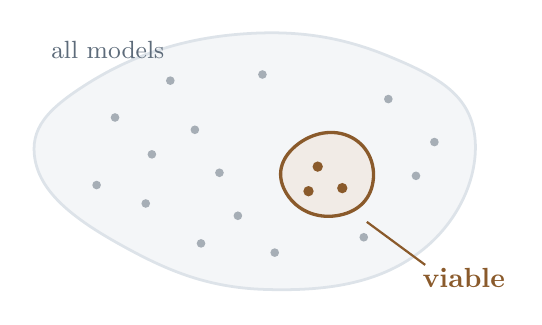
\begin{tikzpicture}[scale=0.78, every node/.style={font=\small}]
      \filldraw[fill=plsurf2, draw=plrule, line width=1pt]
        plot[smooth cycle, tension=0.72] coordinates
          {(0,0) (2.4,0.8) (4.9,0.45) (6.3,-0.8) (5.4,-2.75)
           (2.9,-3.35) (0.5,-2.6) (-0.85,-1.25)};
      \foreach \x/\y in {0.45/-0.55, 1.35/0.05, 2.15/-1.45, 0.95/-1.95,
                         2.85/0.15, 1.75/-0.75, 4.9/-0.25, 5.35/-1.5,
                         4.5/-2.5, 3.05/-2.75, 1.85/-2.6, 0.15/-1.65,
                         2.45/-2.15, 5.65/-0.95, 1.05/-1.15}
        \fill[plmuted!55] (\x,\y) circle (2.0pt);
      \filldraw[fill=plorange!12, draw=plorange, line width=1.2pt]
        plot[smooth cycle, tension=0.85] coordinates
          {(3.35,-1.05) (4.25,-0.85) (4.65,-1.6) (4.05,-2.15) (3.25,-1.8)};
      \foreach \x/\y in {3.75/-1.35, 4.15/-1.7, 3.6/-1.75}
        \fill[plorange] (\x,\y) circle (2.4pt);
      \node[plmuted, anchor=west] at (-0.75,0.55) {all models};
      \draw[plorange, line width=0.8pt] (4.55,-2.25) -- (5.5,-2.95);
      \node[plorange, anchor=north west, font=\bfseries] at (5.3,-2.85) {viable};
    \end{tikzpicture}

    \vspace{6pt}

    {\footnotesize\color{plmuted}
      exclusion plots \;\textbullet\; symmetry constraints
      \;\textbullet\; the swampland\par}

    \vspace{6pt}

    {\color{plnavy}\Large\bfseries Combinatorial explosion\par}
  \end{center}
  \vfill
\end{frame}

%%%%%%%%%%%%%%%%%%%%%%%%%%%%%%%%%%%%%%%%%%%%%%%%%%%%%%%%%%%%%%%%%%%%%%%%%%%%%%%
%  0.6  TYPICAL WAY THESE PROBLEMS ARE APPROACHED
%%%%%%%%%%%%%%%%%%%%%%%%%%%%%%%%%%%%%%%%%%%%%%%%%%%%%%%%%%%%%%%%%%%%%%%%%%%%%%%
\begin{frame}{Typical way these problems are approached}
  \vfill
  \begin{center}
    {\fontsize{18}{22}\selectfont\color{plink}%
      Use a computer algebra system (in practice,
      {\bfseries\color{plnavy}Mathematica}) to either:\par}
  \end{center}
  \vspace{8pt}
  \begin{center}
    \begin{minipage}{0.80\textwidth}
      \raggedright
      \plnum{plorange}{1}{run a brute-force scan}
      \vspace{8pt}
      \plnum{plorange}{2}{use a series of constructions to lift to the right answer}

      \vspace{5pt}

      \onslide<2->{%
        {\fontsize{13}{17}\selectfont\itshape\color{plmuted}%
          I have written these scans. The code was long, unchecked,
          and used exactly once.\par}}
    \end{minipage}
  \end{center}
  \vfill
\end{frame}

%%%%%%%%%%%%%%%%%%%%%%%%%%%%%%%%%%%%%%%%%%%%%%%%%%%%%%%%%%%%%%%%%%%%%%%%%%%%%%%
%  0.8  A CONTROVERSIAL CLAIM  (was: my big question / one solution / that system)
%%%%%%%%%%%%%%%%%%%%%%%%%%%%%%%%%%%%%%%%%%%%%%%%%%%%%%%%%%%%%%%%%%%%%%%%%%%%%%%
\begin{frame}{A controversial claim}
  \vfill
  \begin{center}
    \begin{minipage}{0.86\textwidth}
      \begin{center}
        {\fontsize{20}{27}\selectfont\bfseries\color{plnavy}%
          It would be better to use an\\[2pt]
          {\fontsize{24}{31}\selectfont\color{plorange}interactive
           theorem prover}\\[4pt]
          than a computer algebra system\\[2pt]
          to solve these sorts of problems.\par}
      \end{center}
    \end{minipage}
  \end{center}
  \vfill
\end{frame}

%%%%%%%%%%%%%%%%%%%%%%%%%%%%%%%%%%%%%%%%%%%%%%%%%%%%%%%%%%%%%%%%%%%%%%%%%%%%%%%
%  PART 2  --  INTERACTIVE THEOREM PROVERS
%%%%%%%%%%%%%%%%%%%%%%%%%%%%%%%%%%%%%%%%%%%%%%%%%%%%%%%%%%%%%%%%%%%%%%%%%%%%%%%
{
\setbeamertemplate{background}{\plBackgroundDark}
\setbeamertemplate{footline}{}
\begin{frame}[plain]
  \plpartbody{2}{\plparttitleB}{the tool}
\end{frame}
}

%%%%%%%%%%%%%%%%%%%%%%%%%%%%%%%%%%%%%%%%%%%%%%%%%%%%%%%%%%%%%%%%%%%%%%%%%%%%%%%
%  THE PLAN  (part 2 runs as a debate: what it is / defence / case against)
%%%%%%%%%%%%%%%%%%%%%%%%%%%%%%%%%%%%%%%%%%%%%%%%%%%%%%%%%%%%%%%%%%%%%%%%%%%%%%%
\begin{frame}{The plan}
  \vfill
  \begin{center}
    \begin{minipage}{0.80\textwidth}
      \raggedright
      \plnum{plblue}{1}{What is an interactive theorem prover?}
      \vspace{12pt}
      \plnum{plgreen}{2}{The defence of the claim.}
      \vspace{12pt}
      \plnum{pldel}{3}{The case against the claim.}
      \vspace{12pt}
      \plnum{plorange}{4}{The compromise.}
    \end{minipage}
  \end{center}
  \vfill
\end{frame}

%%%%%%%%%%%%%%%%%%%%%%%%%%%%%%%%%%%%%%%%%%%%%%%%%%%%%%%%%%%%%%%%%%%%%%%%%%%%%%%
%  1.2  WHAT AN ITP IS
%%%%%%%%%%%%%%%%%%%%%%%%%%%%%%%%%%%%%%%%%%%%%%%%%%%%%%%%%%%%%%%%%%%%%%%%%%%%%%%
%  The definition used in the other talks (see ../IAMP.html).
\begin{frame}{What is an interactive theorem prover?}
  \vfill
  \begin{center}
    \begin{plplain}[width=0.86\textwidth, top=12pt, bottom=12pt]{plgreen}
      {\fontsize{17}{23}\selectfont\itshape\color{plink}%
        A programming language in which you can write mathematical theorems
        proofs, and definitions, with mathematical
        {\bfseries\upshape\color{plnavy}correctness} and
        {\bfseries\upshape\color{plnavy}consistency} guaranteed.
        And the definitions you write are
        {\bfseries\upshape\color{plnavy}executable}.\par}
    \end{plplain}
  \end{center}
  \vfill
\end{frame}

%%%%%%%%%%%%%%%%%%%%%%%%%%%%%%%%%%%%%%%%%%%%%%%%%%%%%%%%%%%%%%%%%%%%%%%%%%%%%%%
%  1.3  THE FOUR MAIN ITPS
%%%%%%%%%%%%%%%%%%%%%%%%%%%%%%%%%%%%%%%%%%%%%%%%%%%%%%%%%%%%%%%%%%%%%%%%%%%%%%%
\begin{frame}{The four main interactive theorem provers}
  \vfill
  \begin{columns}[T,onlytextwidth]

    \begin{column}{0.235\textwidth}
      \begin{plcardh}[halign=center, left=4pt, right=4pt]{itprocq}{}{2.0cm}
        \vfill
        {\fontsize{13}{16}\selectfont\bfseries\color{itprocq}Rocq}
        \vfill
      \end{plcardh}
    \end{column}
    \begin{column}{0.235\textwidth}
      \begin{plcardh}[halign=center, left=4pt, right=4pt]{itpisab}{}{2.0cm}
        \vfill
        {\fontsize{13}{16}\selectfont\bfseries\color{itpisab}Isabelle/\allowbreak HOL}
        \vfill
      \end{plcardh}
    \end{column}
    \begin{column}{0.235\textwidth}
      \begin{plcardh}[halign=center, left=4pt, right=4pt]{itplean}{}{2.0cm}
        \vfill
        {\fontsize{13}{16}\selectfont\bfseries\color{itplean}Lean}
        \vfill
      \end{plcardh}
    \end{column}
    \begin{column}{0.235\textwidth}
      \begin{plcardh}[halign=center, left=4pt, right=4pt]{itpagda}{}{2.0cm}
        \vfill
        {\fontsize{13}{16}\selectfont\bfseries\color{itpagda}Agda}
        \vfill
      \end{plcardh}
    \end{column}

  \end{columns}

  \vspace{18pt}
  {\centering\color{plmuted}This talk is in {\bfseries\color{itplean}Lean}.\par}
  \vfill
\end{frame}

%%%%%%%%%%%%%%%%%%%%%%%%%%%%%%%%%%%%%%%%%%%%%%%%%%%%%%%%%%%%%%%%%%%%%%%%%%%%%%%
%  1.4  A RAPID OVERVIEW OF LEAN
%%%%%%%%%%%%%%%%%%%%%%%%%%%%%%%%%%%%%%%%%%%%%%%%%%%%%%%%%%%%%%%%%%%%%%%%%%%%%%%
\begin{frame}[fragile]{A rapid overview of Lean}
  \vfill
  \begin{columns}[c,onlytextwidth]

    \begin{column}{0.455\textwidth}
      \begin{plcard}[top=5pt,bottom=5pt,before skip=2pt]{plblue}{Built on type theory}
        \small
        Lean knows the \textbf{type} of everything, and checks
        that things have the type expected.\par
        \vspace{6pt}
        {\centering\small
          $\underbrace{p}_{\text{proof}}\,:\,\underbrace{P}_{\text{theorem}}
           \qquad
           \underbrace{7}_{\text{term}}\,:\,\underbrace{\mathbb{N}}_{\text{type}}$\par}
      \end{plcard}
    \end{column}

    \begin{column}{0.525\textwidth}
      \begin{plplain}{plorange}
        {\footnotesize\bfseries\color{plorange}A definition, a theorem, a proof}
        \vspace{6pt}
\begin{lstlisting}
def energy (m v : Real) : Real :=
  m * v ^ 2 / 2

theorem energy_nonneg
    (m v : Real) (hm : 0 <= m) :
    0 <= energy m v := by
  unfold energy
  positivity
\end{lstlisting}
      \end{plplain}
    \end{column}

  \end{columns}
  \vfill
\end{frame}

%%%%%%%%%%%%%%%%%%%%%%%%%%%%%%%%%%%%%%%%%%%%%%%%%%%%%%%%%%%%%%%%%%%%%%%%%%%%%%%
%  MATHLIB
%%%%%%%%%%%%%%%%%%%%%%%%%%%%%%%%%%%%%%%%%%%%%%%%%%%%%%%%%%%%%%%%%%%%%%%%%%%%%%%
\begin{frame}{The main libraries}
  \vfill
  \begin{center}
    \plrepocard{leanprover-community}{mathlib4}%
      {The math library of Lean 4.}{3{,}989}{1{,}635}{776}{2021}
  \end{center}
  \vfill
\end{frame}

%%%%%%%%%%%%%%%%%%%%%%%%%%%%%%%%%%%%%%%%%%%%%%%%%%%%%%%%%%%%%%%%%%%%%%%%%%%%%%%
%  PHYSLIB
%%%%%%%%%%%%%%%%%%%%%%%%%%%%%%%%%%%%%%%%%%%%%%%%%%%%%%%%%%%%%%%%%%%%%%%%%%%%%%%
\begin{frame}{The main libraries}
  \vfill
  \begin{center}
    \plrepocard{leanprover-community}{physlib}%
      {A \emph{community-driven} project to digitalise results from physics
       into Lean.}{717}{176}{106}{2024}
  \end{center}
  \vfill
\end{frame}

%%%%%%%%%%%%%%%%%%%%%%%%%%%%%%%%%%%%%%%%%%%%%%%%%%%%%%%%%%%%%%%%%%%%%%%%%%%%%%%
%  CSLIB
%%%%%%%%%%%%%%%%%%%%%%%%%%%%%%%%%%%%%%%%%%%%%%%%%%%%%%%%%%%%%%%%%%%%%%%%%%%%%%%
\begin{frame}{The main libraries}
  \vfill
  \begin{center}
    \plrepocard{leanprover}{cslib}%
      {The computer science library of Lean.}{683}{190}{48}{2025}
  \end{center}
  \vfill
\end{frame}

%%%%%%%%%%%%%%%%%%%%%%%%%%%%%%%%%%%%%%%%%%%%%%%%%%%%%%%%%%%%%%%%%%%%%%%%%%%%%%%
%  1.5  LEAN, LIVE
%%%%%%%%%%%%%%%%%%%%%%%%%%%%%%%%%%%%%%%%%%%%%%%%%%%%%%%%%%%%%%%%%%%%%%%%%%%%%%%
%  QR is ../Images/LeanLiveQR.png -- regenerate it if the link changes.
\begin{frame}{Lean, live}
  \vfill
  \begin{columns}[c,onlytextwidth]

    \begin{column}{0.42\textwidth}
      \begin{center}
        
\includegraphics[width=4.9cm]{LeanLiveQR.png}
      \end{center}
    \end{column}

    \begin{column}{0.54\textwidth}
      {\fontsize{20}{24}\selectfont\bfseries\color{plnavy}
        Follow along example\par}
      \vspace{6pt}
      \vspace{12pt}
      {\fontsize{17}{21}\selectfont\href{https://live.lean-lang.org/\#codez=JYWwDg9gTgLgBAWQIYwBYBtgCMBQf8GFHEAmApgGaICeAcinAFxwAq1YZTAvHFtXAGdoUangB2SEGQFgkAY04I6KPOSpISJJjXrxASYQ6GBpbu69+QqCNWU4IAK7ptJo4f1uzfQcNE50ZEBAkOA0SAH0kASE5OAAKYKw4GOYXGABKbVC4rISMmJ4c7M1eJIzGHi9LETg8NDJoALgoYDEAczCyAEdskpitZkASQjK4ELgAahKAKiTxuC1pmIBaUZ5YxImSDIXPURGq3zwAekWAQjxQSFhEFAxsc7ESezkYYAA3RWV4ZjYOHBGAHzgAC8yFAIM5Pn84ICBE9kh5jJCcBIpDJ5B9dDZ1MUUp84IjTASVAC4AA6EFggA0KwAfCEoYDSbC5DEsNTglw6Uy4XFUqSsokkGl8Go7I4IYSEW4GWSKRB2XBObLQRAZdyWbwFUqsvEMrEHE5BcK/AEgiFNBEohAYvFehKUMMdYUsHlFeatMF4sVEnIyhVdiM4C0YGDRj6oSMWo9nsAIGJRgB3YBoCPQ4EqxU01MjKAUdCpmE8+PAVCZ7NJVBINqcJ3FMTq1mugp1htFLQ+4WBwMCC5wOPofgAbVC1OZclJLQAVgBRToAXXLZAAHvJ4CX8HUGiAmi12l0ej65vb0tpRhNEtsNnBtssOXF1nMtjNyuYoWI43IIIEws02jhFocOBAA}{%
        \color{plorange}\bfseries\underline{live.lean-lang.org}\;
        \faIcon{external-link-alt}}\par}
    \end{column}

  \end{columns}
  \vfill
\end{frame}

%%%%%%%%%%%%%%%%%%%%%%%%%%%%%%%%%%%%%%%%%%%%%%%%%%%%%%%%%%%%%%%%%%%%%%%%%%%%%%%
%  RELATION TO AI AND MATHS IN THE NEWS
%%%%%%%%%%%%%%%%%%%%%%%%%%%%%%%%%%%%%%%%%%%%%%%%%%%%%%%%%%%%%%%%%%%%%%%%%%%%%%%
\begin{frame}{Relation to AI and maths in the news}
  \vfill
  \begin{columns}[T,onlytextwidth]

    \begin{column}{0.235\textwidth}
      \begin{plcardh}{plorange}{\plchip{plorange}{MAY 2026}}{4.3cm}
        \normalsize\bfseries\color{plnavy}
        The unit-distance\\problem
        \par\vspace{6pt}
        {\footnotesize\normalfont\color{plink}Erd\H{o}s, 1946.\\ Disproved.}
        \par\vfill
        {\scriptsize\normalfont\color{plmuted}OpenAI, internal model}
      \end{plcardh}
    \end{column}

    \begin{column}{0.235\textwidth}
      \begin{plcardh}{plorange}{\plchip{plorange}{JUL 2026}}{4.3cm}
        \normalsize\bfseries\color{plnavy}
        The Jacobian\\conjecture
        \par\vspace{6pt}
        {\footnotesize\normalfont\color{plink}Keller, 1939.\\ Counterexample in $\mathbb{C}^{3}$.}
        \par\vfill
        {\scriptsize\normalfont\color{plmuted}Alpoge, with Claude Fable 5}
      \end{plcardh}
    \end{column}

    \begin{column}{0.235\textwidth}
      \begin{plcardh}{plorange}{\plchip{plorange}{AUG 2026}}{4.3cm}
        \normalsize\bfseries\color{plnavy}
        Ten open\\problems
        \par\vspace{6pt}
        {\footnotesize\normalfont\color{plink}Each with a\\ Lean 4 certificate.}
        \par\vfill
        {\scriptsize\normalfont\color{plmuted}OpenAI ``Astra''}
      \end{plcardh}
    \end{column}

    \begin{column}{0.235\textwidth}
      \begin{plcardh}{plorange}{\plchip{plorange}{AUG 2026}}{4.3cm}
        \normalsize\bfseries\color{plnavy}
        Zeros on the\\critical line
        \par\vspace{6pt}
        {\footnotesize\normalfont\color{plink}$41.6\%\to 67.2\%$.\\ \textbf{Not} a proof of RH.}
        \par\vfill
        {\scriptsize\normalfont\color{plmuted}Anthropic, checked in Lean}
      \end{plcardh}
    \end{column}

  \end{columns}
  \vfill
\end{frame}

%%%%%%%%%%%%%%%%%%%%%%%%%%%%%%%%%%%%%%%%%%%%%%%%%%%%%%%%%%%%%%%%%%%%%%%%%%%%%%%
%  THE DEFENCE  (beat; opens movement 2 of the claim--defence--against arc)
%%%%%%%%%%%%%%%%%%%%%%%%%%%%%%%%%%%%%%%%%%%%%%%%%%%%%%%%%%%%%%%%%%%%%%%%%%%%%%%
{
\setbeamertemplate{background}{\plBackgroundDark}
\setbeamertemplate{footline}{}
\begin{frame}[plain]
  \plbeat{-11}{THE DEFENCE}{%
    \begin{minipage}{0.78\textwidth}
      \begin{center}
        {\color{plondarkm}\fontsize{13}{18}\selectfont\itshape
          ``It would be better to use an interactive theorem prover
          than a computer algebra system to solve these sorts of
          problems.''\par}

        \vspace{0.38cm}

        {\color{plondark}\fontsize{20}{25}\selectfont\bfseries
          Here is why.\par}
      \end{center}
    \end{minipage}}
\end{frame}
}

%%%%%%%%%%%%%%%%%%%%%%%%%%%%%%%%%%%%%%%%%%%%%%%%%%%%%%%%%%%%%%%%%%%%%%%%%%%%%%%
%  THE DEFENCE, IN FIVE POINTS  (speed-up folded into 2; point 5 = scan bypass)
%%%%%%%%%%%%%%%%%%%%%%%%%%%%%%%%%%%%%%%%%%%%%%%%%%%%%%%%%%%%%%%%%%%%%%%%%%%%%%%
\begin{frame}{The defence, in five points}
  \vfill
  \begin{center}
    \begin{minipage}{0.90\textwidth}
      \raggedright
      \onslide<1->{%
      \plnums{plgreen}{1}{Interactive theorem provers give you
        {\color{plgreen}trust}.}
      \plnumsub{every step is machine-checked, so a bug cannot hide}}
      \vspace{2pt}
      \onslide<2->{%
      \plnums{plgreen}{2}{Definitions, lemmas and executable functions in
        one language: the {\color{plgreen}full reasoning} is in the code.}
      \plnumsub{and a slow definition can be swapped for a fast algorithm,
        with a proof they agree}}
      \vspace{2pt}
      \onslide<3->{%
      \plnums{plgreen}{3}{They are {\color{plgreen}AI-safe}.}
      \plnumsub{a feedback loop: AI generates, Lean verifies}}
      \vspace{2pt}
      \onslide<4->{%
      \plnums{plgreen}{4}{Lean is set up in {\color{plgreen}monolithic
        libraries}.}
      \plnumsub{one coherent, composable whole in which everything works
        with everything}}
      \vspace{2pt}
      \onslide<5->{%
      \plnums{plgreen}{5}{Theorems can {\color{plgreen}tame the
        combinatorial explosion}.}
      \plnumsub{intuition becomes theorems that construct the answer,
        where a brute-force scan is infeasible}}
    \end{minipage}
  \end{center}
  \vfill
\end{frame}

%%%%%%%%%%%%%%%%%%%%%%%%%%%%%%%%%%%%%%%%%%%%%%%%%%%%%%%%%%%%%%%%%%%%%%%%%%%%%%%
%  1.7  AI AND LEAN, IN A LOOP
%%%%%%%%%%%%%%%%%%%%%%%%%%%%%%%%%%%%%%%%%%%%%%%%%%%%%%%%%%%%%%%%%%%%%%%%%%%%%%%
\begin{frame}{AI and Lean}
  \vfill
  \begin{center}
    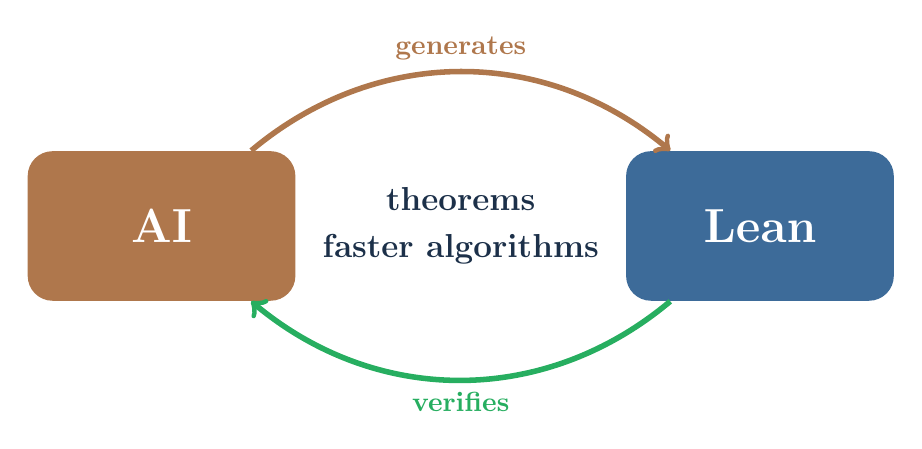
\begin{tikzpicture}[
      box/.style={rounded corners=9pt, text=white, font=\bfseries\LARGE,
                  minimum width=3.4cm, minimum height=1.9cm, align=center},
    ]
      \node[box, fill=fwtan]  (ai)   at (0,0) {AI};
      \node[box, fill=fwblue] (lean) at (7.6,0) {Lean};

      \draw[fwtan, line width=2pt, ->]
        (ai)   to[bend left=40]
        node[above, font=\bfseries, text=fwtan] {generates} (lean);
      \draw[fwgreen, line width=2pt, ->]
        (lean) to[bend left=40]
        node[below, font=\bfseries, text=fwgreen] {verifies} (ai);

      \node[align=center, font=\bfseries\large, text=plnavy] at (3.8,0)
        {theorems\\[3pt] faster algorithms};
    \end{tikzpicture}

  \end{center}
  \vfill
\end{frame}

%%%%%%%%%%%%%%%%%%%%%%%%%%%%%%%%%%%%%%%%%%%%%%%%%%%%%%%%%%%%%%%%%%%%%%%%%%%%%%%
%  THE CASE AGAINST  (beat; movement 3)
%%%%%%%%%%%%%%%%%%%%%%%%%%%%%%%%%%%%%%%%%%%%%%%%%%%%%%%%%%%%%%%%%%%%%%%%%%%%%%%
{
\setbeamertemplate{background}{\plBackgroundDark}
\setbeamertemplate{footline}{}
\begin{frame}[plain]
  \plbeat{11}{THE CASE AGAINST}{%
    {\color{plondark}\fontsize{22}{27}\selectfont\bfseries
      And here is why not.\par}}
\end{frame}
}

%%%%%%%%%%%%%%%%%%%%%%%%%%%%%%%%%%%%%%%%%%%%%%%%%%%%%%%%%%%%%%%%%%%%%%%%%%%%%%%
%  THE CASE AGAINST, IN THREE POINTS
%%%%%%%%%%%%%%%%%%%%%%%%%%%%%%%%%%%%%%%%%%%%%%%%%%%%%%%%%%%%%%%%%%%%%%%%%%%%%%%
\begin{frame}{The case against, in three points}
  \vfill
  \begin{center}
    \begin{minipage}{0.90\textwidth}
      \raggedright
      \onslide<1->{%
      \plnums{pldel}{1}{Decades of work have gone into
        {\color{pldel}computer algebra systems}.}
      \plnumsub{Mathematica, Maple, FORM, and the many other tools built
        by this community}}
      \vspace{10pt}
      \onslide<2->{%
      \plnums{pldel}{2}{So many things a physicist wants to do are
        {\color{pldel}easy in a CAS}.}
      \plnumsub{and, today, not available inside an ITP}}
      \vspace{10pt}
      \onslide<3->{%
      \plnums{pldel}{3}{Adapting these algorithms to an ITP is a
        {\color{pldel}huge amount of work}.}
      \plnumsub{verification is part of the story: the code must come
        with its proof}}
    \end{minipage}
  \end{center}
  \vfill
\end{frame}

%%%%%%%%%%%%%%%%%%%%%%%%%%%%%%%%%%%%%%%%%%%%%%%%%%%%%%%%%%%%%%%%%%%%%%%%%%%%%%%
%  THE COMPROMISE  (beat; movement 4)
%%%%%%%%%%%%%%%%%%%%%%%%%%%%%%%%%%%%%%%%%%%%%%%%%%%%%%%%%%%%%%%%%%%%%%%%%%%%%%%
{
\setbeamertemplate{background}{\plBackgroundDark}
\setbeamertemplate{footline}{}
\begin{frame}[plain]
  \plbeat{0}{THE COMPROMISE}{%
    {\color{plondark}\fontsize{22}{27}\selectfont\bfseries
      Can we get the best\\[2pt] of both worlds?\par}}
\end{frame}
}

%%%%%%%%%%%%%%%%%%%%%%%%%%%%%%%%%%%%%%%%%%%%%%%%%%%%%%%%%%%%%%%%%%%%%%%%%%%%%%%
%  THE BEST OF BOTH WORLDS  (hex: the compromise made concrete)
%%%%%%%%%%%%%%%%%%%%%%%%%%%%%%%%%%%%%%%%%%%%%%%%%%%%%%%%%%%%%%%%%%%%%%%%%%%%%%%
\begin{frame}{We can.}
  \vfill
  \begin{center}
    {\fontsize{16}{20}\selectfont\color{plink}%
      Tactics that do the algebra for you,
      {\bfseries\color{plnavy}verified}:\par}

    \vspace{10pt}

    {\fontsize{24}{28}\selectfont
     {\ttfamily\bfseries\color{plorange}ring}\qquad
     {\ttfamily\bfseries\color{plorange}grind}\par}

    \vspace{6pt}

    {\footnotesize\color{plmuted}\ldots and the beginnings of a verified
     computer algebra library (early days):\par}
    \vspace{2pt}
    \scalebox{0.78}{%
      \plrepocard{leanprover}{hex}%
        {Verified computational algebra in Lean 4: aggregator for the
         released hex libraries.}{21}{2}{2}{2026}}
  \end{center}
  \vfill
\end{frame}

%%%%%%%%%%%%%%%%%%%%%%%%%%%%%%%%%%%%%%%%%%%%%%%%%%%%%%%%%%%%%%%%%%%%%%%%%%%%%%%
%  THE CLAIM, AMENDED  (the compromise lands, feeding the call to action)
%%%%%%%%%%%%%%%%%%%%%%%%%%%%%%%%%%%%%%%%%%%%%%%%%%%%%%%%%%%%%%%%%%%%%%%%%%%%%%%
\begin{frame}
  \vfill
  \begin{center}
    {\fontsize{22}{28}\selectfont\bfseries\color{plorange}%
      Bring the computer algebra\\[2pt]
      into the theorem prover.\par}

    \vspace{16pt}

    {\fontsize{14}{18}\selectfont\color{plmuted}%
      (This is my call to action for this community.)\par}
  \end{center}
  \vfill
\end{frame}

%%%%%%%%%%%%%%%%%%%%%%%%%%%%%%%%%%%%%%%%%%%%%%%%%%%%%%%%%%%%%%%%%%%%%%%%%%%%%%%
%  THE ASK, SHARPENED  (the concrete wish behind the call to action)
%%%%%%%%%%%%%%%%%%%%%%%%%%%%%%%%%%%%%%%%%%%%%%%%%%%%%%%%%%%%%%%%%%%%%%%%%%%%%%%
\begin{frame}
  \vfill
  \begin{center}
    {\fontsize{18}{24}\selectfont\color{plink}%
      In particular, I would love to see, in
      {\bfseries\color{plnavy}Physlib}:\par}

    \vspace{16pt}

    {\fontsize{20}{26}\selectfont\bfseries\color{plorange}%
      tactics and CAS tools that make\\[2pt]
      the physicist's life easier.\par}
  \end{center}
  \vfill
\end{frame}

%%%%%%%%%%%%%%%%%%%%%%%%%%%%%%%%%%%%%%%%%%%%%%%%%%%%%%%%%%%%%%%%%%%%%%%%%%%%%%%
%  PART 3  --  OUR EXPLICIT EXAMPLE
%%%%%%%%%%%%%%%%%%%%%%%%%%%%%%%%%%%%%%%%%%%%%%%%%%%%%%%%%%%%%%%%%%%%%%%%%%%%%%%
{
\setbeamertemplate{background}{\plBackgroundDark}
\setbeamertemplate{footline}{}
\begin{frame}[plain]
  \plpartbody{3}{\plparttitleC}{the proof}
\end{frame}
}

%%%%%%%%%%%%%%%%%%%%%%%%%%%%%%%%%%%%%%%%%%%%%%%%%%%%%%%%%%%%%%%%%%%%%%%%%%%%%%%
%  THE EVIDENCE  (beat; part 3 re-enters the debate)
%%%%%%%%%%%%%%%%%%%%%%%%%%%%%%%%%%%%%%%%%%%%%%%%%%%%%%%%%%%%%%%%%%%%%%%%%%%%%%%
{
\setbeamertemplate{background}{\plBackgroundDark}
\setbeamertemplate{footline}{}
\begin{frame}[plain]
  \plbeat{-17}{THE EVIDENCE}{%
    {\color{plondark}\fontsize{20}{26}\selectfont\bfseries
      The defence made five promises.\\[2pt]
      Here they are, in practice.\par}}
\end{frame}
}

%%%%%%%%%%%%%%%%%%%%%%%%%%%%%%%%%%%%%%%%%%%%%%%%%%%%%%%%%%%%%%%%%%%%%%%%%%%%%%%
%  2.1  THE MATHEMATICAL PROBLEM
%%%%%%%%%%%%%%%%%%%%%%%%%%%%%%%%%%%%%%%%%%%%%%%%%%%%%%%%%%%%%%%%%%%%%%%%%%%%%%%
\begin{frame}{The problem, mathematically}
  \vfill
  \begin{columns}[c,onlytextwidth]

    \begin{column}{0.505\textwidth}
      \begin{center}
        {\color{plnavy}\fontsize{24}{28}\selectfont$(q_{H_d},\,q_{H_u},\,Q_5,\,Q_{10})$\par}

        \vspace{6pt}

        \vspace{-2pt}
        {\small\color{plmuted}
          $q_{H_d},\,q_{H_u} \;:\; \mathrm{Option}\ \mathbb{Z}$\\[2pt]
          $Q_5,\,Q_{10} \;:\; \mathrm{Finset}\ \mathbb{Z}$\par}
        \vspace{6pt}
        {\footnotesize\color{plmuted}all drawn from a finite set\par}

        \vspace{12pt}

        {\color{plnavy}\large\bfseries Large. Finite.\par}
      \end{center}
    \end{column}

    \begin{column}{0.465\textwidth}
      \begin{center}
        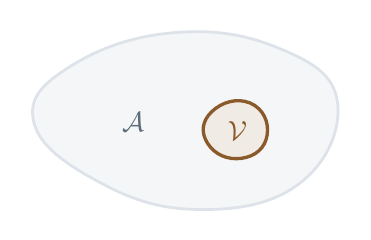
\begin{tikzpicture}[scale=0.54, every node/.style={font=\normalsize}]
          \filldraw[fill=plsurf2, draw=plrule, line width=1pt]
            plot[smooth cycle, tension=0.72] coordinates
              {(0,0) (2.4,0.8) (4.9,0.45) (6.3,-0.8) (5.4,-2.75)
               (2.9,-3.35) (0.5,-2.6) (-0.85,-1.25)};
          \filldraw[fill=plorange!12, draw=plorange, line width=1.2pt]
            plot[smooth cycle, tension=0.85] coordinates
              {(3.35,-1.05) (4.25,-0.85) (4.65,-1.6) (4.05,-2.15) (3.25,-1.8)};
          \node[plmuted] at (1.5,-1.3) {$\mathcal{A}$};
          \node[plorange] at (3.95,-1.5) {$\mathcal{V}$};
        \end{tikzpicture}

        \vspace{6pt}

        {\color{plorange}\large\bfseries Find $\mathcal{V}$.\par}
      \end{center}
    \end{column}

  \end{columns}

  \begin{plplain}[before skip=6pt,top=5pt,bottom=5pt]{plblue}
    {\centering
     {\scriptsize\bfseries\color{plmuted}ONE CONSTRAINT \;\textendash\;
      FORBID THE DANGEROUS COUPLING
      $\overline{\mathbf 5}\,\overline{\mathbf 5}\,\mathbf{10}$}\par
     \vspace{6pt}
     {\large\color{plnavy}$\forall\, a,b \in Q_5,\;\; c \in Q_{10}\;:\qquad
       a + b + c \;\neq\; 0$\par}}
  \end{plplain}
  \vfill
\end{frame}


%%%%%%%%%%%%%%%%%%%%%%%%%%%%%%%%%%%%%%%%%%%%%%%%%%%%%%%%%%%%%%%%%%%%%%%%%%%%%%%
%  2.2  THE PHYSICS -- SU(5) MODEL BUILDING
%%%%%%%%%%%%%%%%%%%%%%%%%%%%%%%%%%%%%%%%%%%%%%%%%%%%%%%%%%%%%%%%%%%%%%%%%%%%%%%
\begin{frame}{The physics: $SU(5)$ model building}
  \vfill
  \begin{columns}[T,onlytextwidth]

    \begin{column}{0.485\textwidth}
      \begin{plcard}[top=6pt,bottom=6pt]{plblue}%
                    {\plchip{plblue}{AMBIENT SPACE}\;$\mathcal{A}$}
        SUSY $SU(5)$ $+$ Abelian symmetry\\[5pt]
        Higgs: down-type, up-type
          \hfill{\color{plorange}$q_{H_d},\,q_{H_u}$}\\[4pt]
        Matter: $\overline{\mathbf 5}$, $\mathbf{10}$
          \hfill{\color{plorange}$Q_5,\,Q_{10}$}\\[5pt]
        {\footnotesize\color{plmuted}charges from finite sets, from F-theory}
      \end{plcard}
    \end{column}

    \begin{column}{0.485\textwidth}
      \begin{plcard}[top=6pt,bottom=6pt]{plorange}%
                    {\plchip{plorange}{VIABLE}\;$\mathcal{V}$}
        Top Yukawa allowed\\[5pt]
        Dangerous operators forbidden\\[5pt]
        No regeneration\\[5pt]
        {\footnotesize\color{plmuted}all conditions on
         $(q_{H_d},q_{H_u},Q_5,Q_{10})$}
      \end{plcard}
    \end{column}

  \end{columns}

  \vfill
\end{frame}

%%%%%%%%%%%%%%%%%%%%%%%%%%%%%%%%%%%%%%%%%%%%%%%%%%%%%%%%%%%%%%%%%%%%%%%%%%%%%%%
%  2.3  LIVES IN PHYSLIB
%%%%%%%%%%%%%%%%%%%%%%%%%%%%%%%%%%%%%%%%%%%%%%%%%%%%%%%%%%%%%%%%%%%%%%%%%%%%%%%
\begin{frame}{Lives in Physlib}
  \vfill
  \begin{center}
    {\color{plmuted}\faIcon{github}\;\texttt{leanprover-community/physlib}\par}

    \vspace{18pt}

    {\ttfamily\fontsize{17}{21}\selectfont\color{plorange}%
      Physlib/Particles/SuperSymmetry/SU5\par}
    \vspace{6pt}
    {\ttfamily\fontsize{17}{21}\selectfont\color{plorange}%
      Physlib/StringTheory/FTheory\par}

    \vspace{24pt}

    {\fontsize{17}{21}\selectfont\color{plink}%
      {\bfseries\color{plnavy}12{,}171 lines} of Lean.\par}
  \end{center}
  \vfill
\end{frame}

%%%%%%%%%%%%%%%%%%%%%%%%%%%%%%%%%%%%%%%%%%%%%%%%%%%%%%%%%%%%%%%%%%%%%%%%%%%%%%%
%  2.4  CODE ORGANIZATION  (paper section 3.5)
%%%%%%%%%%%%%%%%%%%%%%%%%%%%%%%%%%%%%%%%%%%%%%%%%%%%%%%%%%%%%%%%%%%%%%%%%%%%%%%
\begin{frame}{Build an API}
  \vfill
  \begin{columns}[c,onlytextwidth]

    \begin{column}{0.55\textwidth}
      \begin{plplain}[top=3pt,bottom=3pt]{plblue}
        {\ttfamily\fontsize{6.2}{7.3}\selectfont\color{plink}
         {\bfseries\color{plorange}SU5/}\\
         \hspace*{1.1em}FieldLabels.lean\\
         \hspace*{1.1em}Potential.lean\\
         \hspace*{1.1em}{\bfseries\color{plorange}ChargeSpectrum/}\\
         \hspace*{2.4em}Basic.lean\\
         \hspace*{2.4em}OfFieldLabel.lean\\
         \hspace*{2.4em}OfPotentialTerm.lean\\
         \hspace*{2.4em}AllowsTerm.lean\\
         \hspace*{2.4em}{\bfseries\color{plorange}MinimallyAllowsTerm/}\\
         \hspace*{3.7em}Basic.lean\\
         \hspace*{3.7em}FinsetTerms.lean\\
         \hspace*{3.7em}OfFinset.lean\\
         \hspace*{2.4em}MinimalSuperSet.lean\\
         \hspace*{2.4em}Completions.lean\\
         \hspace*{2.4em}PhenoConstrained.lean\\
         \hspace*{2.4em}PhenoClosed.lean\\
         \hspace*{2.4em}Yukawa.lean\\
         \hspace*{2.4em}Map.lean\\
         \hspace*{2.4em}ZMod.lean\par}
      \end{plplain}
    \end{column}

    \begin{column}{0.41\textwidth}
      \begin{plcard}[top=6pt,bottom=6pt]{plorange}{Small pieces}
        Definitions, lemmas, theorems\\[3pt]
        around one data structure\\[3pt]
        composing into the result
      \end{plcard}
    \end{column}

  \end{columns}
  \vfill
\end{frame}

%%%%%%%%%%%%%%%%%%%%%%%%%%%%%%%%%%%%%%%%%%%%%%%%%%%%%%%%%%%%%%%%%%%%%%%%%%%%%%%
%  2.5  FORMAL VOCABULARY  (paper section 3, snippet 1)
%%%%%%%%%%%%%%%%%%%%%%%%%%%%%%%%%%%%%%%%%%%%%%%%%%%%%%%%%%%%%%%%%%%%%%%%%%%%%%%
\begin{frame}[fragile]{Charge spectra as the basic object}
  \vfill
  \begin{center}
    \begin{plplain}[width=0.92\textwidth, top=6pt, bottom=6pt]{plorange}
\begin{lstlisting}[basicstyle=\ttfamily\scriptsize]
structure ChargeSpectrum (𝓩 : Type := ℤ) where
  qHd : Option 𝓩
  qHu : Option 𝓩
  Q5 : Finset 𝓩
  Q10 : Finset 𝓩
\end{lstlisting}
    \end{plplain}

    \vspace{12pt}
    {\color{plmuted}One data structure. Everything else hangs off it.\par}

    \vspace{18pt}

    {\fontsize{16}{20}\selectfont\color{plink}%
      Restrict $q_{H_d}$, $q_{H_u}$, $Q_5$ and $Q_{10}$ to draw from
      finite subsets of $\mathcal{Z}$, and the type becomes
      {\bfseries\color{plnavy}our ambient space $\mathcal{A}$}.\par}
  \end{center}
  \vfill
\end{frame}

%%%%%%%%%%%%%%%%%%%%%%%%%%%%%%%%%%%%%%%%%%%%%%%%%%%%%%%%%%%%%%%%%%%%%%%%%%%%%%%
%  2.6  STRUCTURAL RELATIONS  (paper section 3.2, snippet 2)
%%%%%%%%%%%%%%%%%%%%%%%%%%%%%%%%%%%%%%%%%%%%%%%%%%%%%%%%%%%%%%%%%%%%%%%%%%%%%%%
\begin{frame}[fragile]{Instances}
  \vfill
  \begin{center}
    \begin{plplain}[width=0.92\textwidth, top=6pt, bottom=6pt]{plorange}
\begin{lstlisting}[basicstyle=\ttfamily\scriptsize]
instance emptyInst : EmptyCollection (ChargeSpectrum 𝓩) where
  emptyCollection := ⟨none, none, {}, {}⟩

instance hasSubset : HasSubset (ChargeSpectrum 𝓩) where
  Subset x y :=
    x.qHd.toFinset ⊆ y.qHd.toFinset ∧
    x.qHu.toFinset ⊆ y.qHu.toFinset ∧
    x.Q5 ⊆ y.Q5 ∧
    x.Q10 ⊆ y.Q10
\end{lstlisting}
    \end{plplain}

    \vspace{12pt}
    {\footnotesize\color{plmuted}The whole argument is stated using
     $\subseteq$.\par}
    \vspace{12pt}
    {\fontsize{14}{18}\selectfont\color{plink}Once it is an instance,
     {\bfseries\color{plnavy}Mathlib's lemmas about $\subseteq$ apply.}\par}
  \end{center}
  \vfill
\end{frame}

%%%%%%%%%%%%%%%%%%%%%%%%%%%%%%%%%%%%%%%%%%%%%%%%%%%%%%%%%%%%%%%%%%%%%%%%%%%%%%%
%  2.7  THE VERBS OF THE API  (paper section 3.3)
%%%%%%%%%%%%%%%%%%%%%%%%%%%%%%%%%%%%%%%%%%%%%%%%%%%%%%%%%%%%%%%%%%%%%%%%%%%%%%%
\begin{frame}[fragile]{The verbs of the API}
  \vfill
  \begin{center}
    {\fontsize{14}{18}\selectfont\color{plink}%
      The things you want to ask about, and
      {\bfseries\color{plnavy}the questions you want to ask of them.}\par}

    \vspace{6pt}

    \begin{plplain}[width=0.95\textwidth, top=6pt, bottom=6pt]{plorange}
\begin{lstlisting}[basicstyle=\ttfamily\scriptsize]
def AllowsTerm (x : ChargeSpectrum 𝓩) (T : PotentialTerm) : Prop :=
  0 ∈ ofPotentialTerm x T

def IsPhenoConstrained (x : ChargeSpectrum 𝓩) : Prop :=
  x.AllowsTerm μ ∨ x.AllowsTerm β ∨ x.AllowsTerm Λ ∨ x.AllowsTerm W2 ∨
  x.AllowsTerm W4 ∨ x.AllowsTerm K1 ∨ x.AllowsTerm K2 ∨ x.AllowsTerm W1
\end{lstlisting}
    \end{plplain}

    \vspace{6pt}
    {\fontsize{13}{17}\selectfont\color{plink}%
      {\ttfamily$\neg$\,AllowsTerm x $\Lambda$} is the
      $\forall\,a,b \in Q_5,\, c \in Q_{10}:\, a+b+c \neq 0$ from earlier.
      {\color{plmuted}$\neg$\,\texttt{IsPhenoConstrained} bundles it and
       seven more.}\par}
  \end{center}
  \vfill
\end{frame}

%%%%%%%%%%%%%%%%%%%%%%%%%%%%%%%%%%%%%%%%%%%%%%%%%%%%%%%%%%%%%%%%%%%%%%%%%%%%%%%
%  2.8  STEP 1 -- MINIMAL WITNESSES
%%%%%%%%%%%%%%%%%%%%%%%%%%%%%%%%%%%%%%%%%%%%%%%%%%%%%%%%%%%%%%%%%%%%%%%%%%%%%%%
\begin{frame}[fragile]{Step 1 (theorem): a small set of seeds}
  \vfill
  \begin{columns}[c,onlytextwidth]
    \begin{column}{0.46\textwidth}
      \begin{center}
        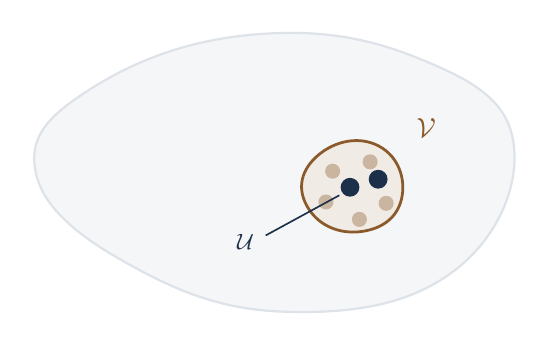
\begin{tikzpicture}[scale=1.70]
          \plblob{%
            \foreach \x/\y in {1.80/-0.62, 2.08/-0.55, 2.20/-0.86,
                               1.75/-0.85, 2.00/-0.98}
              {\fill[plorange!45] (\x,\y) circle (1.6pt);}
            \foreach \x/\y in {1.93/-0.74, 2.14/-0.68}
              {\fill[plnavy] (\x,\y) circle (2.0pt);}}
          \node[plorange] at (2.50,-0.30) {$\mathcal{V}$};
          \node[plnavy, font=\footnotesize] at (1.15,-1.15) {$\mathcal{U}$};
          \draw[plnavy, line width=0.6pt] (1.3,-1.10) -- (1.85,-0.80);
        \end{tikzpicture}
      \end{center}
    \end{column}
    \begin{column}{0.50\textwidth}
      {\fontsize{15}{19}\selectfont\color{plink}%
        Every element of $\mathcal{V}$ contains\\[2pt]
        one of these as a subset.\par}
      \vspace{12pt}
      \begin{plplain}[top=4pt,bottom=4pt]{plblue}
\begin{lstlisting}[basicstyle=\ttfamily\fontsize{6.7}{8.0}\selectfont]
lemma allowsTerm_iff_subset_minimallyAllowsTerm :
    x.AllowsTerm T ↔
    ∃ y ∈ powerset x, y.MinimallyAllowsTerm T
\end{lstlisting}
      \end{plplain}
    \end{column}
  \end{columns}
  \vfill
\end{frame}

%%%%%%%%%%%%%%%%%%%%%%%%%%%%%%%%%%%%%%%%%%%%%%%%%%%%%%%%%%%%%%%%%%%%%%%%%%%%%%%
%  2.9  STEP 2 -- WHICH ADDITIONS ARE ALLOWED
%%%%%%%%%%%%%%%%%%%%%%%%%%%%%%%%%%%%%%%%%%%%%%%%%%%%%%%%%%%%%%%%%%%%%%%%%%%%%%%
\begin{frame}[fragile]{Step 2 (theorem): which additions are allowed}
  \vfill
  \begin{columns}[c,onlytextwidth]
    \begin{column}{0.46\textwidth}
      \begin{center}
        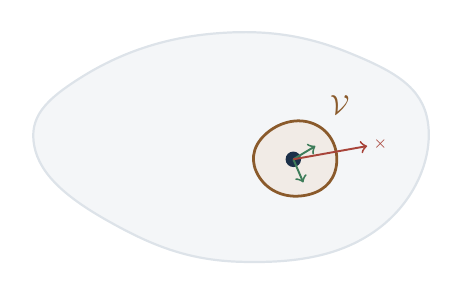
\begin{tikzpicture}[scale=1.40]
          \plblob{%
            \fill[plnavy] (1.93,-0.74) circle (2.0pt);
            \draw[plgreen, line width=0.7pt, ->] (1.93,-0.74) -- (2.13,-0.62);
            \draw[plgreen, line width=0.7pt, ->] (1.93,-0.74) -- (2.02,-0.95);
            \draw[pldel, line width=0.7pt, ->]   (1.93,-0.74) -- (2.60,-0.62);
            \node[pldel, font=\tiny] at (2.72,-0.60) {$\times$};}
          \node[plorange] at (2.35,-0.25) {$\mathcal{V}$};
        \end{tikzpicture}
      \end{center}
    \end{column}
    \begin{column}{0.50\textwidth}
      {\fontsize{13}{17}\selectfont\color{plink}%
        Add a charge to $Q_5$ or $Q_{10}$,
        or fill in $q_{H_d}$ or $q_{H_u}$.\par}
      \vspace{4pt}
      {\color{plgreen}\bfseries Some additions stay inside $\mathcal{V}$.}\\[3pt]
      {\color{pldel}\bfseries Some leave it.}
      \vspace{6pt}
      \par{\fontsize{13}{17}\selectfont\color{plnavy}\bfseries
       And once you leave,\\ you cannot get back in.\par}
      \vspace{6pt}
      \begin{plplain}[top=4pt,bottom=4pt]{plblue}
\begin{lstlisting}[basicstyle=\ttfamily\fontsize{7.0}{8.4}\selectfont]
lemma isPhenoConstrained_mono
    {x y : ChargeSpectrum 𝓩} (h : x ⊆ y)
    (hx : x.IsPhenoConstrained) :
    y.IsPhenoConstrained
\end{lstlisting}
      \end{plplain}
    \end{column}
  \end{columns}

  \vfill
\end{frame}

%%%%%%%%%%%%%%%%%%%%%%%%%%%%%%%%%%%%%%%%%%%%%%%%%%%%%%%%%%%%%%%%%%%%%%%%%%%%%%%
%  2.10  STEP 3 -- AN EXPLICIT TEST
%%%%%%%%%%%%%%%%%%%%%%%%%%%%%%%%%%%%%%%%%%%%%%%%%%%%%%%%%%%%%%%%%%%%%%%%%%%%%%%
\begin{frame}{Step 3 (theorem): a classification}
  \vfill
  \begin{center}
    {\fontsize{16}{20}\selectfont\color{plink}%
      Steps 1 and 2 give {\bfseries\color{plnavy}easy-to-check}
      conditions on $\mathcal{V}$:\par}

    \vspace{12pt}

    \begin{plplain}[width=0.80\textwidth, halign=center,
                    top=9pt, bottom=9pt]{plorange}
      {\fontsize{17}{21}\selectfont\color{plnavy}%
        $x \in \mathcal{V}$\quad$\iff$\quad
        {\bfseries viability conditions on $x$}\par}
    \end{plplain}

  \end{center}
  \vfill
\end{frame}

%%%%%%%%%%%%%%%%%%%%%%%%%%%%%%%%%%%%%%%%%%%%%%%%%%%%%%%%%%%%%%%%%%%%%%%%%%%%%%%
%  2.11  STEP 4 -- COMPUTE A CANDIDATE
%%%%%%%%%%%%%%%%%%%%%%%%%%%%%%%%%%%%%%%%%%%%%%%%%%%%%%%%%%%%%%%%%%%%%%%%%%%%%%%
\begin{frame}{Step 4 (compute): $\mathcal{V}_0$}
  \vfill
  \begin{columns}[c,onlytextwidth]
    \begin{column}{0.44\textwidth}
      \begin{center}
        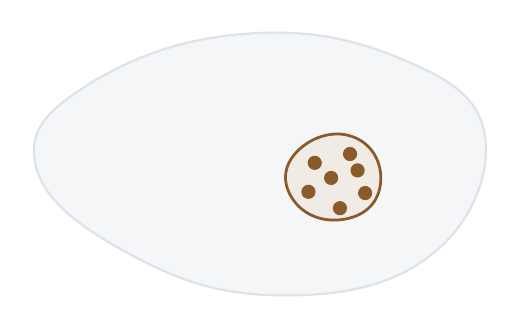
\begin{tikzpicture}[scale=1.60]
          \plblob{%
            \foreach \x/\y in {1.80/-0.62, 2.08/-0.55, 2.20/-0.86, 1.75/-0.85,
                               2.00/-0.98, 1.93/-0.74, 2.14/-0.68}
              {\fill[plorange] (\x,\y) circle (1.6pt);}}
        \end{tikzpicture}
      \end{center}
    \end{column}
    \begin{column}{0.52\textwidth}
      {\fontsize{16}{20}\selectfont\color{plink}%
        Run the construction with\\[2pt]
        ordinary techniques.\par}
      \vspace{12pt}
      {\color{plnavy}\bfseries Out comes a list, $\mathcal{V}_0$.\par}
      \vspace{12pt}
      {\footnotesize\color{plmuted}\texttt{completeMinSubset}\quad
       \texttt{minimalSuperSet}\quad \texttt{viableCharges}\par}
    \end{column}
  \end{columns}

  \vfill
\end{frame}

%%%%%%%%%%%%%%%%%%%%%%%%%%%%%%%%%%%%%%%%%%%%%%%%%%%%%%%%%%%%%%%%%%%%%%%%%%%%%%%
%  2.12  STEP 5 -- CERTIFY IT
%%%%%%%%%%%%%%%%%%%%%%%%%%%%%%%%%%%%%%%%%%%%%%%%%%%%%%%%%%%%%%%%%%%%%%%%%%%%%%%
\begin{frame}[fragile]{Step 5 (theorem): $\mathcal{V}_0 = \mathcal{V}$}
  \vfill
  \begin{columns}[T,onlytextwidth]
    \begin{column}{0.465\textwidth}
      \begin{plcardh}[top=5pt,bottom=5pt]{plblue}%
                     {\plchip{plblue}{STEP 3}}{1.35cm}
        \centering$x \in \mathcal{V}\;\iff\;$viability conditions
      \end{plcardh}
    \end{column}
    \begin{column}{0.465\textwidth}
      \begin{plcardh}[top=5pt,bottom=5pt]{plorange}%
                     {\plchip{plorange}{STEP 4}}{1.35cm}
        \centering$\mathcal{V}_0$, a list you can print
      \end{plcardh}
    \end{column}
  \end{columns}

  \vspace{8pt}
  {\centering{\color{plgreen}\fontsize{20}{20}\selectfont$\Downarrow$}\par}
  \vspace{8pt}

  \begin{center}
    \begin{plplain}[width=0.90\textwidth, top=5pt, bottom=5pt]{plgreen}
\begin{lstlisting}[basicstyle=\ttfamily\fontsize{6.9}{8.3}\selectfont]
lemma mem_viableCharges_iff {I} {x : ChargeSpectrum}
    (hsub : x ∈ ofFinset I.allowedBarFiveCharges I.allowedTenCharges) :
    x ∈ viableCharges I ↔
      AllowsTerm x topYukawa ∧
      ¬ IsPhenoConstrained x ∧
      ¬ YukawaGeneratesDangerousAtLevel x 1 ∧
      IsComplete x := ...
\end{lstlisting}
    \end{plplain}
  \end{center}
  \vfill
\end{frame}

%%%%%%%%%%%%%%%%%%%%%%%%%%%%%%%%%%%%%%%%%%%%%%%%%%%%%%%%%%%%%%%%%%%%%%%%%%%%%%%
%  2.13  THE PAYOFF -- the defence's promises, made good by the example
%%%%%%%%%%%%%%%%%%%%%%%%%%%%%%%%%%%%%%%%%%%%%%%%%%%%%%%%%%%%%%%%%%%%%%%%%%%%%%%
\begin{frame}{The claims made good}
  \vfill
  \begin{center}
    \begin{minipage}{0.86\textwidth}
      \raggedright
      \onslide<1->{%
      \plnums{plgreen}{1}{{\color{plgreen}Trust}: the final theorem is certified.}
      \plnumsub{$\mathcal{V}_0 = \mathcal{V}$, every step checked, so a
        bug cannot hide}}
      \vspace{2pt}
      \onslide<2->{%
      \plnums{plgreen}{2}{{\color{plgreen}Full reasoning}: the argument lives in the code.}
      \plnumsub{the lemmas you just saw are the physicist's intuition,
        made precise}}
      \vspace{2pt}
      \onslide<3->{%
      \plnums{plgreen}{3}{{\color{plgreen}AI-safe}: AI could have written this code.}
      \plnumsub{with Lean checking every line}}
      \vspace{2pt}
      \onslide<4->{%
      \plnums{plgreen}{4}{{\color{plgreen}Monolithic libraries}: the API
        now lives in Physlib.}
      \plnumsub{12{,}171 lines, ready for the next project to build on}}
      \vspace{2pt}
      \onslide<5->{%
      \plnums{plgreen}{5}{{\color{plgreen}Combinatorial explosion}: we never had to scan.}
      \plnumsub{$\mathcal{V}_0$ was built up from minimal seeds, then
        certified}}
    \end{minipage}
  \end{center}
  \vfill
\end{frame}

%%%%%%%%%%%%%%%%%%%%%%%%%%%%%%%%%%%%%%%%%%%%%%%%%%%%%%%%%%%%%%%%%%%%%%%%%%%%%%%
%  CONCLUSION
%%%%%%%%%%%%%%%%%%%%%%%%%%%%%%%%%%%%%%%%%%%%%%%%%%%%%%%%%%%%%%%%%%%%%%%%%%%%%%%
\begin{frame}{In conclusion}
  \vfill
  \begin{center}
    \begin{minipage}{0.86\textwidth}
      \raggedright
      {\fontsize{18}{24}\selectfont\color{plink}%
        I have made a {\bfseries\color{plnavy}controversial claim}.
        You do not need to believe it.\par}

      \vspace{22pt}

      {\fontsize{18}{24}\selectfont\color{plink}%
        But I hope you take away some of the
        {\bfseries\color{plorange}benefits} of interactive theorem
        provers, and some of the things you can
        {\bfseries\color{plorange}do} with them.\par}
    \end{minipage}
  \end{center}
  \vfill
\end{frame}

%%%%%%%%%%%%%%%%%%%%%%%%%%%%%%%%%%%%%%%%%%%%%%%%%%%%%%%%%%%%%%%%%%%%%%%%%%%%%%%
%  CLOSING
%%%%%%%%%%%%%%%%%%%%%%%%%%%%%%%%%%%%%%%%%%%%%%%%%%%%%%%%%%%%%%%%%%%%%%%%%%%%%%%
{
\setbeamertemplate{background}{\plBackgroundDark}
\setbeamertemplate{footline}{}
\begin{frame}[plain]
  \vfill
  \begin{center}
    {\color{plondark}\fontsize{36}{40}\selectfont\bfseries
      Thank you for watching\par}

    \vspace{0.50cm}

    
\begin{tikzpicture}
      \fill[plondarkm!55!pldarkbg] (0,0) rectangle (2.5cm,2pt);
      \fill[plondarka] (2.75cm,-3pt) circle (4.5pt);
      \fill[plondarkm!55!pldarkbg] (3.2cm,0) rectangle (5.7cm,2pt);
    \end{tikzpicture}

    \vspace{0.50cm}

    {\color{plondarkm}\normalsize Joseph Tooby-Smith\par}

    \vspace{0.40cm}

    {\color{plondarkm}\footnotesize
      \href{https://github.com/leanprover-community/physlib}{%
        \color{plondarkm}\faIcon{github}\; \texttt{leanprover-community/physlib}}
      \qquad
      \href{https://josephtoobysmith.com/}{%
        \color{plondarkm}\faIcon{globe}\; \texttt{josephtoobysmith.com}}\par}
  \end{center}
  \vfill
\end{frame}
}

\end{document}
